\section{Code}
NOTE: Links are not directly shown here since the urls contain the author name. They are shown in full at the linked bibliography entry.

Code available at \cite{webmga_3_github}. Live program accessible at \cite{webmga_3_app}.

\section{User Manual}
\begin{lstlisting}
                _       __     __    __  ____________
               | |     / /__  / /_  /  |/  / ____/   |
               | | /| / / _ \/ __ \/ /|_/ / / __/ /| |
               | |/ |/ /  __/ /_/ / /  / / /_/ / ___ |
               |__/|__/\___/_.___/_/  /_/\____/_/  |_|

                 by Eduardo Battistini, Yue He, REDACTED

====================================================================
                           USER MANUAL
====================================================================

Welcome to WebMGA.

Please see the 'About' section of the program to learn more about
the purpose of WebMGA and the configurations included in the
Library.

~~~~~~~~~~~~~~~~~~~~~~~~~~~~~~~~~~~~~~~~~~~~~~~~~~~~~~~~~~~~~~~~~~~~
                             LICENSE
~~~~~~~~~~~~~~~~~~~~~~~~~~~~~~~~~~~~~~~~~~~~~~~~~~~~~~~~~~~~~~~~~~~~

Copyright 2024. Carlos Eduardo Battistini Parra, Yue He, REDACTED.

Permission is hereby granted, free of charge, to any person
obtaining a copy of this software and associated documentation files
(the "Software"), to deal in the Software without restriction,
including without limitation the rights to use, copy, modify, merge,
publish, distribute, sublicense, and/or sell copies of the Software,
and to permit persons to whom the Software is furnished to do so,
subject to the following conditions:

The above copyright notice and this permission notice shall be
included in all copies or substantial portions of the Software.

THE SOFTWARE IS PROVIDED "AS IS", WITHOUT WARRANTY OF ANY KIND,
EXPRESS OR IMPLIED, INCLUDING BUT NOT LIMITED TO THE WARRANTIES
OF MERCHANTABILITY, FITNESS FOR A PARTICULAR PURPOSE AND
NONINFRINGEMENT. IN NO EVENT SHALL THE AUTHORS OR COPYRIGHT HOLDERS
BE LIABLE FOR ANY CLAIM, DAMAGES OR OTHER LIABILITY, WHETHER IN AN
ACTION OF CONTRACT, TORT OR OTHERWISE, ARISING FROM, OUT OF OR IN
CONNECTION WITH THE SOFTWARE OR THE USE OR OTHER DEALINGS IN THE
SOFTWARE.

~~~~~~~~~~~~~~~~~~~~~~~~~~~~~~~~~~~~~~~~~~~~~~~~~~~~~~~~~~~~~~~~~~~~
                     CONFIGURATION FILE FORMAT
~~~~~~~~~~~~~~~~~~~~~~~~~~~~~~~~~~~~~~~~~~~~~~~~~~~~~~~~~~~~~~~~~~~~

To upload a custom configuration, you may upload a .cnf format
file, or generate a JSON file containing positions, orientations,
and sets of molecules in the following format and upload it.

{
    "model": {
        "sets": [
            {
                "name": "Set A",
                "orientationType": "v",
                "positions": [
                    [0,0,0]
                ],
                "orientations": [
                    [0,1,0]
                ]
            }
        ]
    }
}


For information on the JSON format, please see:
https://www.json.org/

If your configuration has more than one molecule type, restrict each
set of molecules to a different object in the "sets" list.

You may name sets as you please.

You must identify which format you are specifying the molecule
orientations with for the "orientationType" with one of the following
identifiers:

	v - Unit vector
	q - Quaternion
	a - Axis angles
	e - Euler angles

Each molecule should have a corresponding position and orientation
list in the lists "positions" and "orientations".

~~~~~~~~~~~~~~~~~~~~~~~~~~~~~~~~~~~~~~~~~~~~~~~~~~~~~~~~~~~~~~~~~~~~
                    ORIENTATION SPECIFICATION
~~~~~~~~~~~~~~~~~~~~~~~~~~~~~~~~~~~~~~~~~~~~~~~~~~~~~~~~~~~~~~~~~~~~

Unit Vector: [x,y,z]
Quaternion : [w,x,y,z]
Euler angles: [x,y,z]
Axis angles: [axis_x, axis_y, axis_z, angle]

~~~~~~~~~~~~~~~~~~~~~~~~~~~~~~~~~~~~~~~~~~~~~~~~~~~~~~~~~~~~~~~~~~~~
                         .WEBMGA FILES
~~~~~~~~~~~~~~~~~~~~~~~~~~~~~~~~~~~~~~~~~~~~~~~~~~~~~~~~~~~~~~~~~~~~

If you save a configuration, the provided model data will be saved
in JSON format along with a "view" object, which contains all the
viewing parameters at the time the configuration was saved. You may
change the parameters manually in the saved file or re-upload this
type of file to recreate a model with specified viewing settings.

To see a sample, please select a configuration from the Library and
click 'Save'.

~~~~~~~~~~~~~~~~~~~~~~~~~~~~~~~~~~~~~~~~~~~~~~~~~~~~~~~~~~~~~~~~~~~~
                        SUB-MENU OVERVIEW
~~~~~~~~~~~~~~~~~~~~~~~~~~~~~~~~~~~~~~~~~~~~~~~~~~~~~~~~~~~~~~~~~~~~

The menu in the header contains information about WebMGA, Uploading,
Saving, Exporting, and Uploading, as well as the Library of preset
configurations and level of detail (LOD) setting.

By increasing the LOD, more detailed images will be produced at the
cost of poorer performance.

In the Sidebar, you will find the following sub-menus:

Model:

For picking a shape for each of the sets in the configurations and
its corresponding parameters. Also includes options for colouring
manually or by the mesophase director and displaying shapes as
wireframes.

Ambient:

For specifying ambient light and background colours.

Lighting:

For specifying positions and colours of 'point' and 'directional'
lights. Toggling 'helpers' will display figures that will make
positioning lights easier.

Slicing:

For clipping the system in X, Y, or Z dimensions. Also includes
'helpers'.

Reference:

For including a grid, axes (which may be coloured using the
director), and a bounding shape. The size and colour of the grid
and axes may be specified. Periodic folding or repetition may also
be enabled and configured.

~~~~~~~~~~~~~~~~~~~~~~~~~~~~~~~~~~~~~~~~~~~~~~~~~~~~~~~~~~~~~~~~~~~~
                             CONTACT
~~~~~~~~~~~~~~~~~~~~~~~~~~~~~~~~~~~~~~~~~~~~~~~~~~~~~~~~~~~~~~~~~~~~

For help, queries, suggestions or anything else, please contact
REDACTED

====================================================================
                    THANK YOU FOR USING WEBMGA!
====================================================================
\end{lstlisting}

\section{Key Commands}
Key commands are summarised in \cref{tab:dev_help}.
\begin{table}[!h]
  \begin{center}
    \begin{tabular}{ll}
    \hline\hline
       npm run-script build & Build program. \\
       npm run-script start & Run program on local server and open. \\
       npm run-script deploy & Deploy to GitHub page configured in package.json.\\
       \hline\hline
    \end{tabular}
  \end{center}
  \caption{Key commands for development}
  \label{tab:dev_help}
\end{table}

\section{Project proposal}
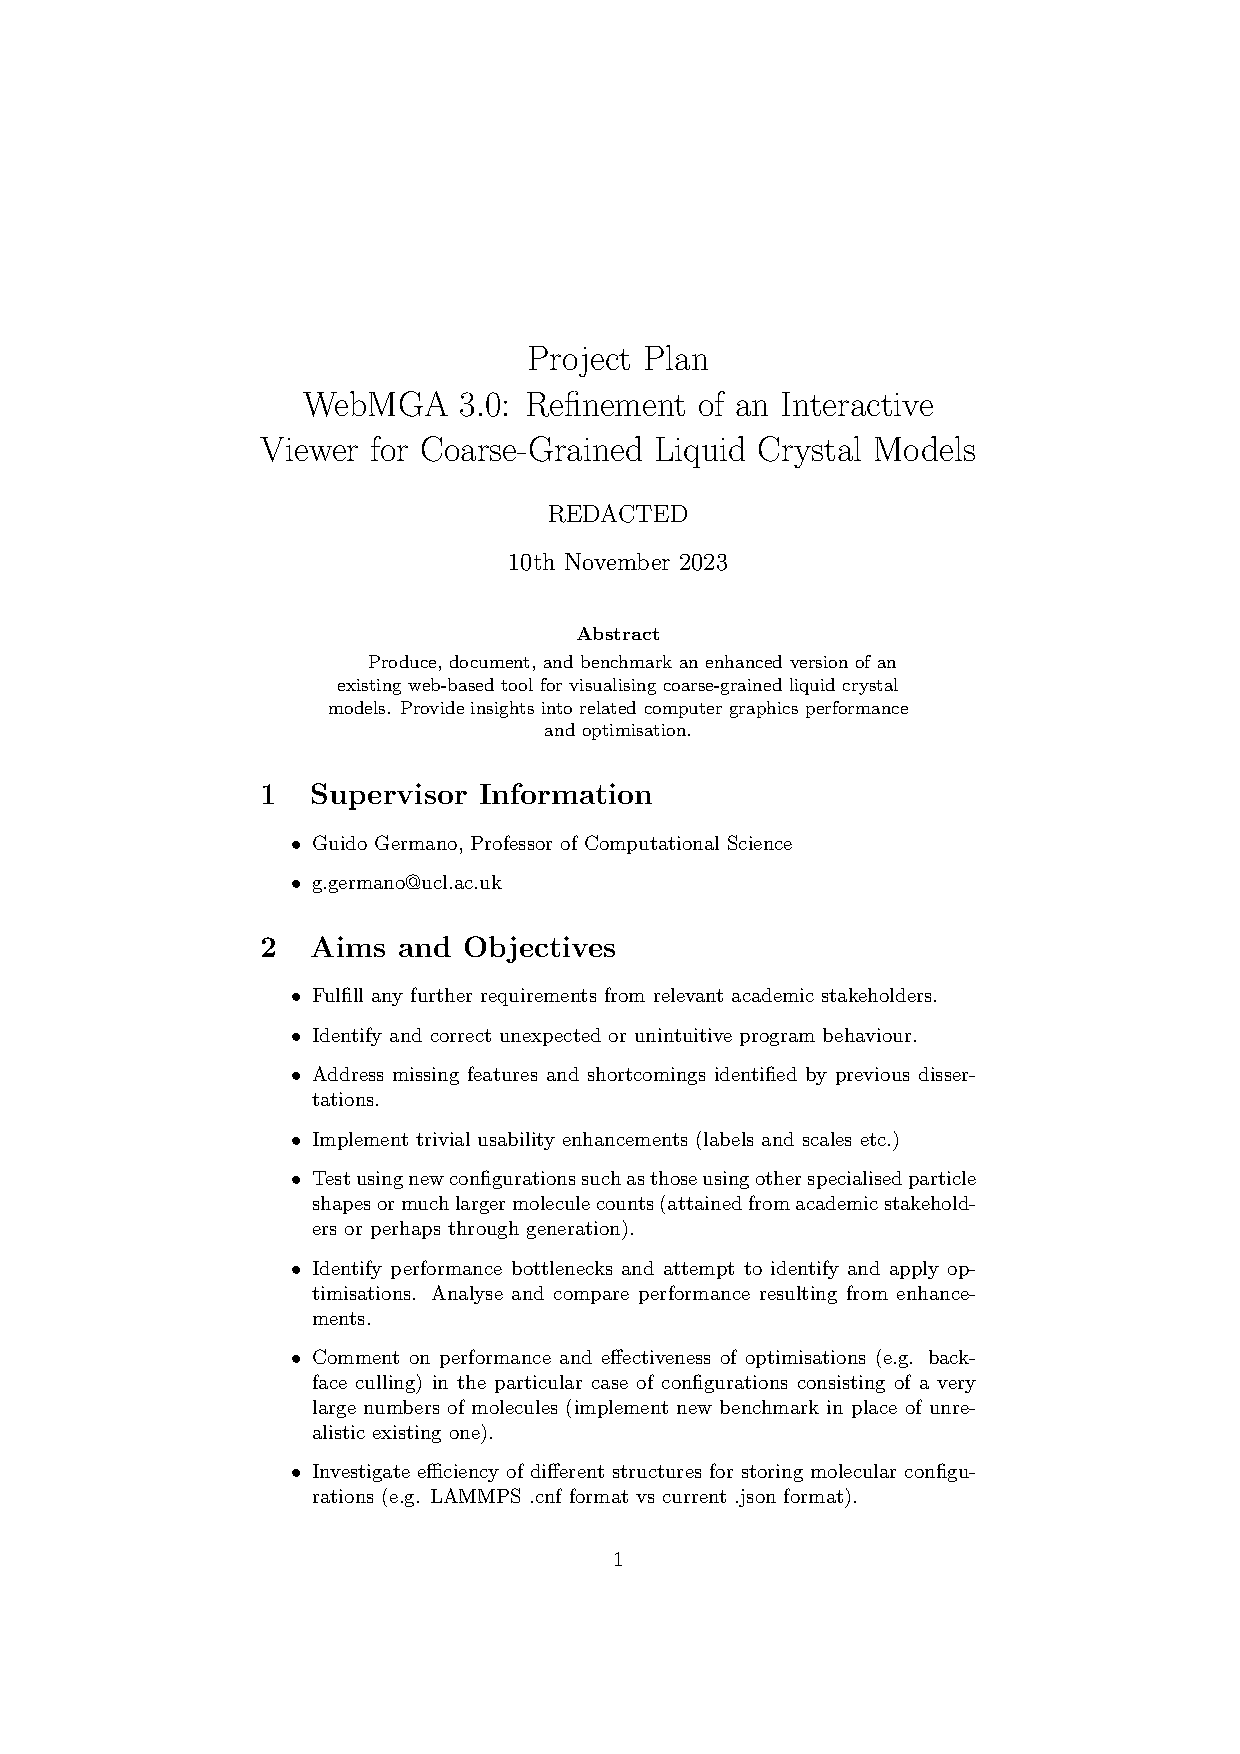
\includepdf[pages=-]{assets/progress_reports/proposal.pdf}

\section{Interim Report}
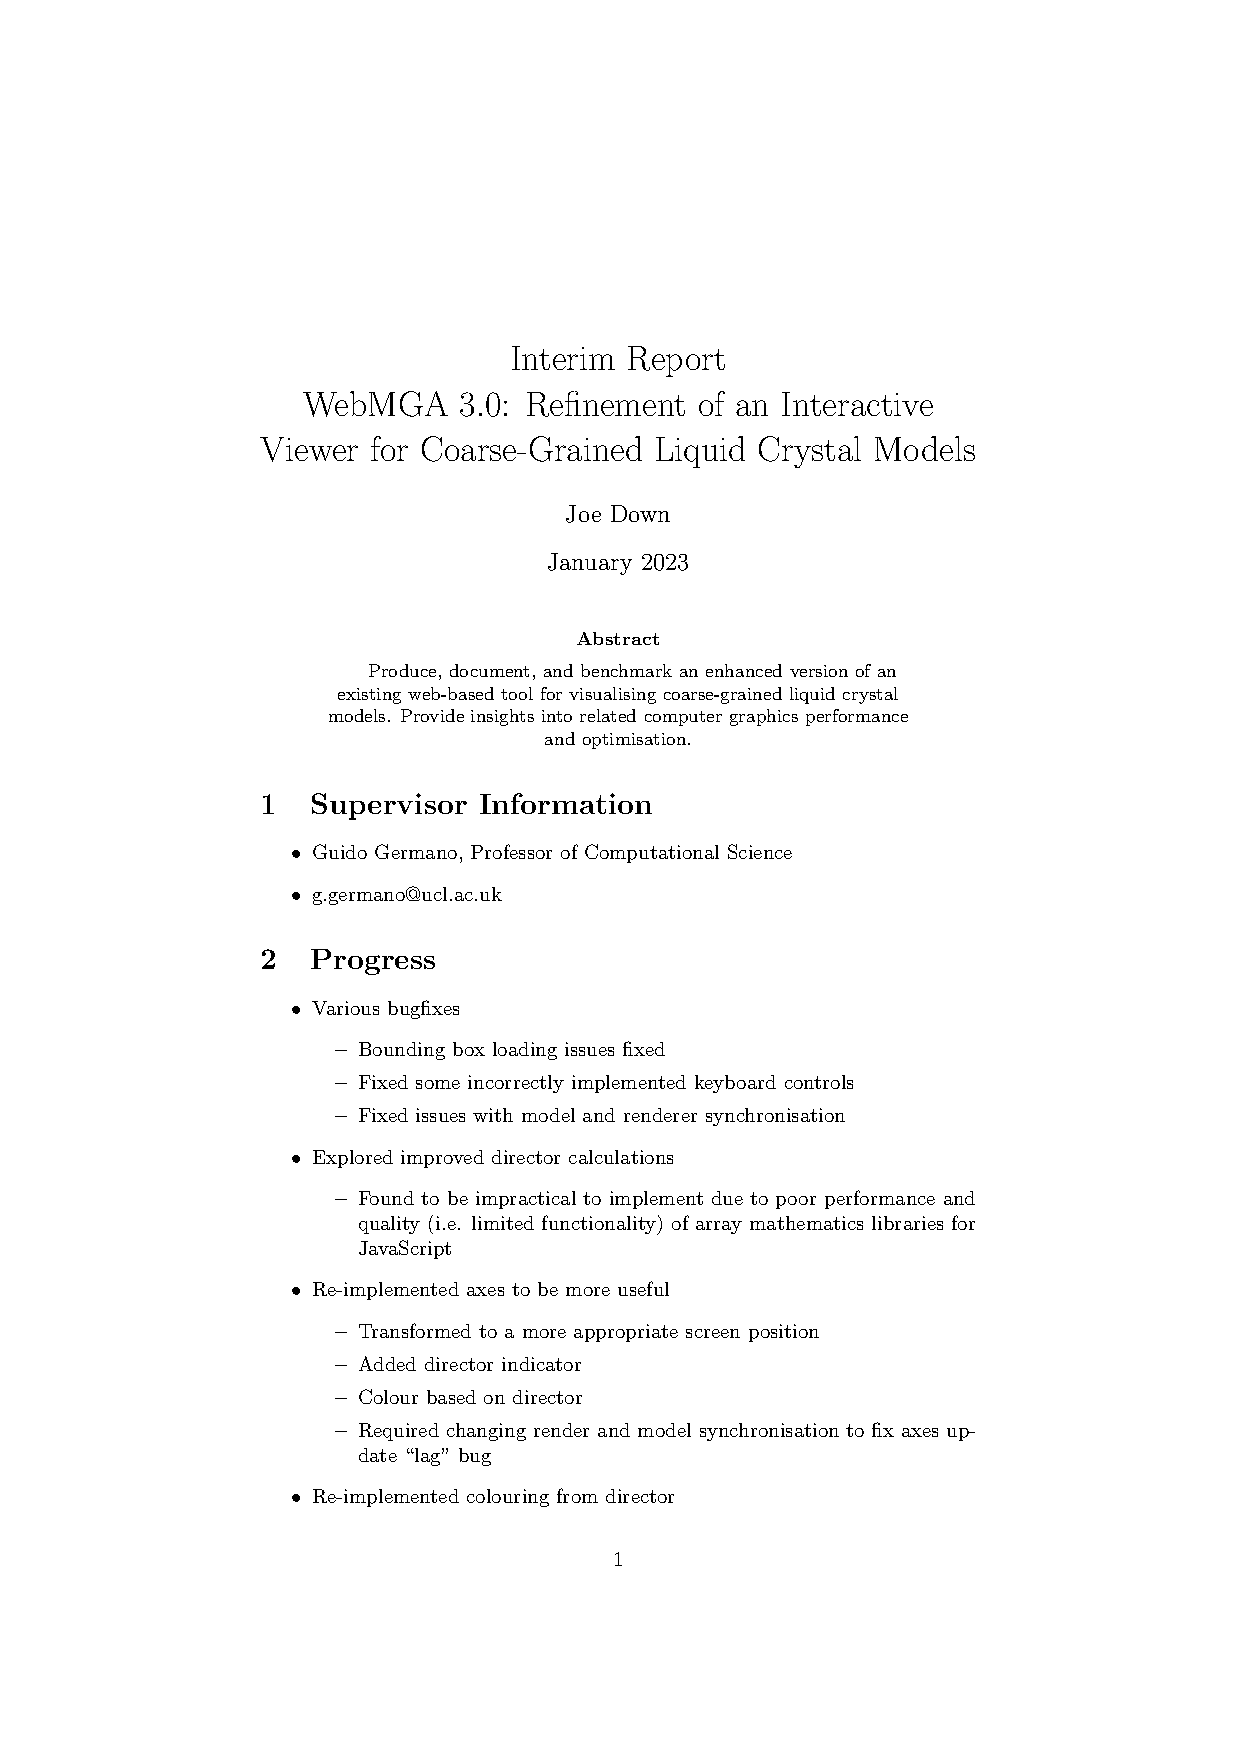
\includepdf[pages=-]{assets/progress_reports/interim.pdf}
